\documentclass{amsbook}

\usepackage[utf8]{inputenc}
\usepackage{parskip}
\usepackage{amssymb}
\usepackage{amsthm}

\usepackage{pgf}
\usepackage{tkz-graph}
\usepackage{tikz}
\usetikzlibrary{arrows,automata,cd,positioning,shapes}

\newtheorem{definition}{Definition}[section]
\newtheorem{lemma}{Lemma}[section]
\newtheorem{theorem}{Theorem}[section]

\newcommand{\dderives}[1]{\mbox{\,$\Rightarrow_{#1}$\,}}
\newcommand{\derives}[1]{\mbox{\,$\stackrel{*}{\Rightarrow}_{#1}$\,}}

\begin{document}

\title{
	Formal Languages\\
	An automata-theoretic introduction}

\author{
	G\"unter Hotz\\
	Universit\"at des Saarlandes
\and
	Klaus Estenfeld\\
	Universit\"at des Saarlandes
\and
	Armin Reichert\\
	Alumnus Universit\"at des Saarlandes\\
	English Translation
}

\maketitle

\chapter*{Preface}

This book is meant to be the second edition of the book Hotz/Walter:
''Automatentheorie und Formale Sprachen II, Endliche Automaten''.

\transrem{English title would be ''Automata theory and formal languages II,
finite automata''.}

But as the book has been completely reworked, it may really be taken as a
completely new one.

While in the first edition only the theory of finite automata has been treated,
in this edition also an introduction into the theory of context-free languages
is given. This was only possible in the available space frame because
of an automata-theoretic treatment of the theory.

Such a foundation of the theory has already been proposed by Goldstine in 1977
and has been sketched in various talks. The motivation for developing
my lecture (from which this book originates) in that way is however not based on
his proposal. It almost automatically arose from dealing with the works of the
French school.

\transrem{With the ''French school'' the works of Schützenberger, Nivat, Perrot,
Sakarovitch, Berstel et al.\ are referred to.}

I must emphasize here the book by Jean Berstel on
transductions. Mr.\ Berstel finally pointed my to the work of Goldstine. I fully
support Goldstine's opinion that it would be worth rethinking the whole theory of formal languages along this automata-theoretic lines.

This book is only an introduction into the theory of formal languages. The
interested reader who wants to gets a deeper understanding of the theory or who
wants to get a different look into it is pointed to the books by Ginsburg,
Harrison or Salomaa. Relations to applications can be found in books on compiler
design.

Dr.\ Klaus Estenfeld worked out my lecture ''Formal Languages I'' which I held 
on this topic in the winter semester of 1980/81 to become the foundation of this
book and he made a number of additions at some places.

Dipl.-Math.\ Bernd Becker carefully read the manuscript and contributed with his
proposals to the success of this book.

The publisher as well as the editors of the series earn our thanks for their
patience of waiting for the second edition.

Saarbrücken, August 1981

\vspace{1em}
{\em Günter Hotz}

\tableofcontents
\chapter*{Introduction}

There are several reasons for the interest in the theory of formal languages in
computer science. Practical problems as they arise in the context of definition
and translation of programming languages find an exact description in the theory
of formal languages and thus get accessible to an exact treatment. Generation
processes definable by formal languages can be interpreted as non-deterministic
automata which is as a generalized notion of a computer.

These kinds of generalizations in general are easier to understand than
deterministic algorithms which contain more details that do not reflect the
original problem but the necessity to uniquely define the algorithm. This is
part of the reason for the difficulty to prove the correctness of programs in an
understandable way. The proof of correctness for grammars or other mechanisms for generating
languages on the other side offers the possibility to study correctness proofs
on simpler objects.

The theory of formal languages in this respect contains the theory of
algorithms but most often only the theory of context-free languages is treated
because of her extraordinary simplicity and beauty.

In the spotlight of the theory are different methods for defining
formal language classes, to study their word and equivalence problems and to
put them into different hierarchical classifications.

The generation processes themselves become objects of interest in the theory
because the generation process of a language in case of programming languages
relates to the semantics of programs.

Of course, in the context of such a pocket book we have to make a strong
selection of topics concerning language classes, generation processes as well as
basic questions. In doing so, we let us guide by the intention to keep the
formal machinery rather small.

Because the theory of finite automata is the foundation for the whole theory of
formal languages, we start our book with this topic. In developing this theory
we do not consider the technical realization of finite automata by logical
circuits and binary storage devices but rather focus on the basic algorithm however it is realized.
 
Our intuitive notion of finite automaton consists of a finite, oriented graph whose 
edges are labeled with the symbols from the input alphabet of the automaton. 
Depending on the input word, we look for a path in the graph labeled with that
word. If the end point of such a path, originating from the dedicated ''start point'' 
of the automaton, is a member of the set of ''end points'', our automaton
''accepts'' the word and doesn't so otherwise.

We prove the equivalence of this concept with the other known methods of
defining finite automata. We prove the usual closure properties of languages
defined by finite automata. Additionally we investigate the relation between
deterministic and non-deterministic automata and also 2-way automata.

It is possible to generalize this theory in the direction of considering not
only the free monoid of strings (words) over a finite alphabet but also
arbitrary monoids.

By considering finite automata with output, which means to attach a second label
at the graph edges, we get the theory of rational transducers. An extensive
treatment of the theory of general transductions can be found in the book by
Berstel.

Here we restrict ourselves to some special generalizations of the free monoid
(of words), namely the {\bf free group}, the {\bf H-group} (where the relation
$x x^{-1} = 1$ holds for $x$ from the generating system, but not $x^{-1} x = 1$) and the
{\bf polycyclic monoid} (in addition to $x x^{-1} = 1$ it holds $x y^{-1} = 0$
for $x \neq y$ and $0 x = x 0 = 0$ for $x,y$ from the generating system).

By investigating the transductions from free monoids into the polycyclic
monoids one gets a smooth transition from the theory of finite automata into the
theory of context-free languages.

The corresponding construction of the theory of context-free languages leads to
a simple path to the most important representation theorems. This includes the
theorems of Chomsky-Schützenberger, Shamir and Greibach. Also for the
transformation into Greibach normal form we get a simple and efficient
algorithm.

In the same easy way as for finite automata you can prove the known closure
properties for context-free languages.

In the end we also prove the equivalence of this representation with the usual
representation of context-free languages using context-free grammars.

Our composition of the theory is very close to the one repeatedly recommended by
Goldstine since 1977, but its origin is independent from him. The difference is
that we prove Greibach's representation theorem by making our automaton deterministic,
namely by switching from output monoids to monoid rings. Doing that you get the
theorem of Shamir in a natural way and from this the theorem of Greibach.

From the theorem of Shamir you can get quite easily the algorithm of Valiant for
deciding the word problem of context-free languages. Because of lack of space
this could not be included into this book, the same holds for the treatment of
the  deterministic languages.

We want to emphasize another advantage of this composition of the theory: As
known, the exact formalization of the notion of ''derivation'' when using
grammars brings some difficulties. In our theory, the ''derivation tree''
corresponds to a path in our graph.

Maybe the use of non-free monoids is initially a problem for readers not used to
it. But it seems to be the case that defining context-free
languages in that way supports the intuition. For example, the usage of ''syntax
diagrams'' for the definition of programming languages gives some evidence for
this.

Because we judge the former as rather important, we want to explain it on a
specific example, namely the so-called {\bf Dyck language}.

The {\bf Dyck language} $D(X_k)$ contains the correctly nested bracket sequences
over $k$ different pairs of brackets, where $k \in \mathbb{N}$.

A formal definition of $D(X_k)$ is as follows:

Let $X_k = \{ x_1, \ldots, x_k \}$ be an alphabet of $k$ elements. Define
$\bar{X}_k = \{ \bar{x}_1, \ldots, \bar{x}_k \}$ such that $\bar{x}_i$ is regarded as the
closing bracket for $x_i$.

Then it holds:

\begin{enumerate}
  \item $\epsilon \in D(X_k)$
  \item $u, v \in D(X_k) \Rightarrow u \cdot v \in D(X_k)$
  \item $u \in D(X_k) \Rightarrow x_i \cdot u \cdot \bar{x}_i \in D(X_k),\quad
  \forall i = 1, \ldots, k$
  \item $D(X_k)$ is minimal with (1), (2) and (3). 
\end{enumerate}

For $D(X_k)$ we get the following syntax diagram:

\begin{center}
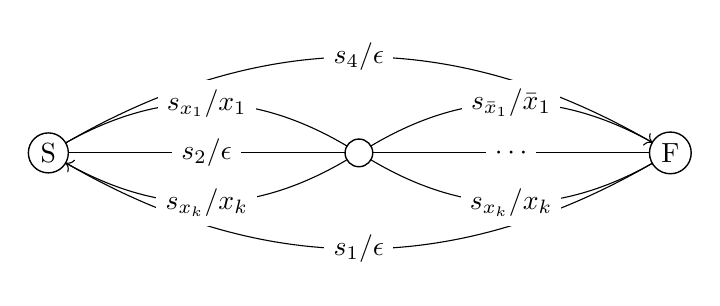
\begin{tikzpicture}[node distance = 10em]
\tikzset{VertexStyle/.append style = {minimum size = 1em}}
\tikzset{EdgeStyle/.append style = {->, bend left}}
\tikzset{LabelStyle/.style = {fill=white}}
\node[VertexStyle](S){S};
\node[VertexStyle,right=of S](V){ }; 
\node[VertexStyle,right=of V](F){F};
\draw[EdgeStyle](S) to node[LabelStyle]{$s_4/\epsilon$} (F);
\draw[EdgeStyle](F) to node[LabelStyle]{$s_1/\epsilon$} (S);
\path[]
	(S)	edge[bend left] 	node[LabelStyle] {$s_{x_1}/x_1$} (V)
	(S)	edge 							node[LabelStyle] {$\cdots$} (V)
	(S)	edge[bend right] 	node[LabelStyle] {$s_{x_k}/x_k$} (V)
	(V)	edge[bend left] 	node[LabelStyle] {$s_{\bar{x}_1}/\bar{x}_1$} (F)
	(V)	edge 							node[LabelStyle] {$\cdots$} (F)
	(V)	edge[bend right] 	node[LabelStyle] {$s_{x_k}/x_k$} (F)
	(V) edge							node[LabelStyle] {$s_2/\epsilon$} (S)
	;
\end{tikzpicture}
\end{center}

If we consider all labelings of paths from $S$ to $F$ we get of course also
words not contained in $D(X_k)$, for example $x_1 x_2 \bar{x}_k$ or $x_1
\bar{x}_1 \bar{x}_2$ etc.

We have to guarantee that we get Dyck words only. To do that, we define a
homomorphism from the path category of the graph into the polycyclic monoid over
$X_k \cup \bar{X}_k$ such that the homomorphic images of the paths from $S$ to
$F$ have a special form, for example to be equal to the unit of the
polycyclic monoid.

Let us consider the word
\[ x_1 x_2 \bar{x}_2 \bar{x}_1 x_2 \bar{x}_2 \in D(X_2), \]
then we have different paths
\[s_{x_1} s_2 s_{x_2} s_{\bar{x}_2} s_3 s_{\bar{x}_1} s_1
s_{x_2} s_{\bar{x}_2} \] 
and 
\[s_{x_1} s_2 s_{x_2} s_{\bar{x}_2} s_3
s_{\bar{x}_1} s_3 s_2 s_{x_2} s_{\bar{x}_2}\]
which both have this word as their labeling and we can easily define a
homomorphism in the sense above.

We get different paths in our graph leading to acceptance of the same word.

The problem to construct a graph such that for each word in the accepted
language exactly one path exists leads to the existence of the {\bf
deterministic} finite automaton with storage.


\chapter{Mathematical foundations}
\section{Notations, basic notions}

In this first section we want to define the elementary notions that are used
throughout the whole book. We use the usual notions
\[ \mathbb{N} = \{ 0, 1, 2, \ldots \}\ \mbox{for the natural numbers} \]
\[ \mathbb{Z} = \{ \ldots, -2, -1, 0, 1, 2, \ldots \}\ \mbox{for the integer
numbers} \]
\[ \mathbb{Q} = \{ \frac{a}{b} \mid a,b \in \mathbb{Z}, b \neq 0 \}\ \mbox{for
the rational numbers } \]

For the set operations we use $\cup$ for the union and $\cap$ for the
intersection. Also $A \subset B$, $a \in A$, $a \not\in A$, $\bar{A}$, $A - B$,
$A \times B$ and $\emptyset$ have their usual meaning. For the power set of a
set $A$ we write $2^A$ or $Pot(A)$. $Card(A)$ denotes the cardinality of $A$.
Logical implication is denoted by $\Rightarrow$.

{\bf Mappings} are denoted as $f : A \rightarrow B$, in that case $f$ is a
total mapping. We write $Q(f) = A, Z(f) = B$. Here $Q$ stands for ''Quelle'' (source)
and $Z$ for ''Ziel'' (target).

If $f: A \rightarrow B, g : B \rightarrow C$ are mappings, then $f \circ g : A
\rightarrow C$ is the composed mapping that one gets by applying $f$ first and
then $g$, i.e. $(f \circ g)(a) = g(f(a))$. If $f:A \rightarrow B$ and $C
\subset A$, then $f(C) = \{ f(c) \mid c \in C \}$.

A subset $R \subset A \times B$ is called a {\bf relation} between $A$ and $B$.
$R_f \subset A \times B$ with $R_f = \{ (a,b) \mid f(a) = b \}$ is the relation
{\bf induced by} mapping f or the {\bf graph} of $f$.

Let $f : A \rightarrow B$ be a mapping, $A_1 \subset A$ and $g : A_1 \rightarrow
B$ a mapping. $f$ is called the {\bf continuation} of $g$ if $f(a_1) = g(a_1),
a_1 \in A_1$. In this case we also write $f \mid _{A_1} = g$ (in words: $f$
restricted to $A_1$).

A {\bf semi-group} consists of a set $M$ an an associative operation on that
set, usually denoted as a multiplication. If a semi-group is commutative, we
also use ''$+$'' instead of ''$\cdot$''.

A semi-group is a {\bf monoid} if $M$ contains a neutral element. We often
denote it with $1_M$ or shortly $1$. In the commutative case we often write $0$
instead of $1$.

For $A,B \subset M$ we denote by $A \cdot B = \{ a b \mid a \in A, b \in B \}$
the {\bf complex product} of $A$ and $B$.

$A \subset M$ is a {\bf submonoid} of $M$ if the follwoing holds: $1_M \in A$
and $A$ is closed under the operation of $M$.

For an $A$, the set $A^*$ defined as follows, is the smallest submonoid of $M$
which contains $A$. More specific,
\[
		A^* = \bigcap_{M' \in M(A)} M'	
\]
where $M(A) = \{ M' \subset M \mid M'$ is a submonoid of $M, A \subset M' \}$.

It is easy to see that
\[
		A^* = \bigcup_{n \geq 0} A^n\ \mbox{with}\ A^0 = \{1\}\ \mbox{and}\ A^{n+1} =
		A^n \cdot A
\]

In the same sense the notion $A^+ = A^* - \{1\}$ is defined for semi-groups. $A$
is called the {\bf generation system} of $A^*$ and $A^+$ resp.

A special meaning for us is assigned to the set of ''words'' (string) over a
fixed alphabet $A$. We understand as words the finite sequences of elements from
the alphabet $A$ as for example $(a,b,d,a,c)$ for alphabet $A = \{ a,b,c,d \}$.

We define
\[
WORD(A) := \{\epsilon\} \cup A \cup (A \times A) \cup (A \times A \times A) \cup
\ldots
\]
as the set of words (strings) over $A$. The symbol $\epsilon$ denotes the {\bf
empty word} over $A$, that is $A^0 = \{\epsilon\}$.

If $w, v \in WORD(A)$ then $w \cdot v$ is the word over $A$ which you get by
concatenating $w$ and $v$, more formally:
\[
\mbox{If}\ w = (a_1,\ldots,a_k), v = (a_{k+1},\ldots,a_n)\ \mbox{then}\ w \cdot
v = (a_1, \ldots, a_n)
\]

With this operation $WORD(A)$ becomes a monoid which is usually also denoted
with $A^*$. This is slightly inconsistent because for the first definition of
the $*$-operator it holds $(A^*)^* = A^*$ but for the second usage of the
$*$-operator it holds $(A*)^* \neq A^*$.

The following example should clarify that: Let $A = \{a,b,c\}$ and let $(a,b,a)$
and $(b,a) \in A^*$.
\[(a,b,a)\cdot(b,a) = (a,b,a,b,a) \in A^*,\ \mbox{but}\]
\[((a,b,a),(b,a)) \in (A^*)^*\ \mbox{but}\ \notin A^*\].


Instead of $(a)$ we write just $a$. In this sense it holds $A \subset A^*$. This
also holds in the sense of the first definition of $A^*$.

If $w = (w_1,\ldots,w_n)$ we denote with $|a| = n$ the {\bf length} of $w$.
Obviously it holds: $|w \cdot v| = |w| + |v|$ and $|\epsilon| = 0$.

The {\bf mirror word} $w^R$ of a word $w = (w_1,\ldots,w_n)$ is the word
$(w_n,\ldots,w_1)$. $\epsilon^R = \epsilon$. It holds: $(w \cdot v)^R =
v^R \cdot w^R$.

In $A^*$ the reduction rules hold, i.e.
\begin{enumerate}
  \item $w \cdot x = w \cdot y \Rightarrow x = y$
  \item $x \cdot w = y \cdot w \Rightarrow x = y$
\end{enumerate}

We define {\bf left} and {\bf right quotient}:
\[ B^{-1} \cdot A = \{ v\ |\ \exists u \in B, w \in A : u \cdot v = w \} \]
and $A \cdot B^{-1}$ in the same way.

Because of the reduction rules it holds:
\[ \{w\}^{-1} \cdot \{v\}\ \mbox{and}\ \{w\}^{-1} \cdot \{v\}\ \mbox{resp. are
either empty or contain a single element.} \]

If $\{w\}^{-1} \cdot \{v\}$ is not empty we call $w$ a {\bf prefix} of $v$. If
$\{w\} \cdot \{v\}^{-1} \not= \emptyset $, we call $v$ a {\bf suffix} of $w$. In
the future we will always write just $w$ instead of $\{w\}$ and also $w$ is
prefix of $v$ if $w^{-1} \cdot v \not= \emptyset$.


\section{Monoid homomorphisms and congruence relations}

\begin{definition}[monoid homomorphism]
A {\bf monoid homomorphism} (short: homomorphism) from a monoid $M$ to a monoid
$S$ is a mapping $\Phi : M \to S$ with the following properties:
\begin{enumerate}
  \item $\Phi(m_1 \cdot m_2) = \Phi(m_1) \cdot \Phi(m_2), \quad m_1, m_2 \in M$
  \item $\Phi(1_M) = 1_S$
\end{enumerate}
\end{definition}

It can be easily shown: if $M_1 \subset M$ is a submonoid of $M$, then
$\Phi(M_1)$ is a submonoid of $S$. If $S_1$ is a submonoid of $S$, then
$\Phi^{-1}(S_1)$ is a submonoid of $M$.

A monoid homomorphism $\Phi : M \to S$ is called
\begin{description}
  \item[monomorphism] if $\Phi$ is injective
  \item[epimorphism] if $\Phi$ is surjective
  \item[isomorphism] if $\Phi$ is bijective
\end{description}

Homomorphisms $\Phi : M \to M$ are called {\bf endomorphisms}, isomorphisms
$\Phi : M \to M$ are called {\bf automorphisms}.

Monoids $M$ and $S$ are called {\bf isomorphic}, if there exists an
isomorphism between $M$ and $S$.

Of course, a homomorphism cannot be defined arbitrarily on a monoid $M$.
Thus the following two questions arise:
\begin{enumerate}
  \item If $M_1 \subset M$ is a submonoid and $\Phi_1 : M_1 \to S$ is an arbitrary
mapping. When is it possible to extend $\Phi_1$ to a homomorphism $\Phi
: M \to S$\ ?
	\item If $\Phi_1, \Phi_2$ both are homomorphisms from $M$ to $S$ which
	coincide on $M_1 \subset M$. In which way can $\Phi_1$ and $\Phi_2$ be
	different? 
\end{enumerate}

The answer to this question of course depends on the structure of $M_1$. If
$M_1 = \{ 1_M \}$ then $\Phi$ is determined uniquely on $M_1$ but there is
little information on the relation between $\Phi_1$ and $\Phi2$.

The following two simple theorems which can be found in introductory algebra
books are holding:
\begin{enumerate}
  \item If $M_1$ is a generating system of $M$ and $\Phi_1, \Phi_2 : M \to S$
  both are monoid homomorphisms which coincide on $M_1$, then $\Phi1 = \Phi_2$.
  \item If $A$ is a set and $M = A^*$, and $\Phi_1 : A \to S$ is an arbitrary
  mapping, then there exists exactly one continuation $\Phi$ from $\Phi_1$ which
  is a monoid homomorphism from $A^*$ to $S$.
\end{enumerate}

\begin{definition}[free generating system, free monoid]
A subset $A \subset M$ is called a {\bf free generating system} of $M$, if each
mapping $\Phi_1 : A \to S$, where $S$ is an arbitrary monoid, can be continued
to a monoid homomorphims in a unique way. A monoid with a free generating system
is called a {\bf free monoid}.
\end{definition}

$A^*$ therefore is a free monoid and $A$ is a free generating system of $A^*$.

It holds also: If $A$ is a free generating system of $M$ and $A^*$ is the monoid
of words (string) over $A$, then $A^*$ and $M$ are isomorphic.

A free monoid has at most one free generating system. From that we can see that
the length $|w|$ of a word $w \in A^*$ can be defined in a unique way for any
free monoid.

The length mapping $L$ is an example for a monoid homomorphism $L : A^* \to
\mathbb{N}$.

If $\Phi : M \to S$ is a monoid homomorphism, then the sets 
\[\{ \Phi^{-1}(s) \mid s \in S \} \subset Pot(M)\]
form a monoid isomorphic to $\Phi(M)$.

We want to handle now the following question:

Let $M$ be a monoid, $L \subset M$ be any subset of $M$. Does there exist a
monoid $S$ and a homomorphism $\Phi : M \to S$ with the following property:
There exists an $s \in S$ with $L \subset \Phi^{-1}(s)$?

Of course, there always exists such an $S$: Choose $S = \{1\}$ and $\Phi(M) =
\{1\}$.

Therefore we strengthen our task: Find $S$ and $\Phi$ such that $L \subset
\Phi^{-1}(S)$ and for each other homomorphism $\Psi$ with that property holds:
$L \subset \Psi^{-1}(S') \Rightarrow \Phi^{-1}(S) \subset \Psi^{-1}(S')$.

We want to describe $L$ as close as possible by a monoid homomorphism.

Such an $S$ and $\Phi$ exists for each $L \subset M$ (see Algebra text), it is
named $synt_M(L)$ an is constructed as follows:

\begin{definition}[syntactic congruence]
Let $M$ be a monoid and $L \subset M$. For $a, b \in M$ we define
\[ a \equiv b\ (L) \Leftrightarrow \mbox{for all}\ u, v \in M: u \cdot a \cdot v
\in L \Leftrightarrow u \cdot b \cdot v \in L
\]
\end{definition}

$\equiv (L)$ is a congruence relation, it holds:
\begin{enumerate}
  \item Let $[a]_L = \{ b \in M \mid a \equiv b\ (L) \}$\ then\ $b \in [a]_L
  \Rightarrow [a]_L = [b]_L $
  \item If we define $[a]_L \cdot [b]_L := [a b]_L$\ (complex product), then
  \[synt_M(L) = \{ [a]_L \mid a \in M \}\] becomes a monoid and the mapping
  \[\Psi_L : M \to synt_M(L),\ \Psi_L(a) = [a]_L\]
   is a monoid epimorphism.
\end{enumerate}

We call $\equiv (L)$ the {\bf syntactic congruence} of $L$ and $synt_M(L)$ the
{\bf syntactic monoid} of $L$ wrt. $M$.

To motivate the name ''syntactic monoid'' we give an example from German
language.
Let $A$ be the alphabet of German and $L$ the set of sentences in German. One can
denote two words $w_1$ and $w_2$ as congruent if they can always be exchanged in
each german sentence. There exist words that cannot always be exchanged. In the
sentence ''Apfel ist eine Kernfrucht'' the word ''Apfel'' can be exchanged by
''Birne'' but this is not possible in the sentence ''Apfel schreibt sich A p f e
l''.

The difficulty is of semantic nature. If you don't consider semantic correctness
of sentences you get a classification of words wrt. their syntactic meaning.

The important notion of ''syntactic congruence'' has been introduced by M. P.
Schützenberger in the context of coding problems.

\section{Special monoids and the free group}

We have just learned about the syntactic monoid as an example for a monoid.
Further information on the theory of syntactic monoids can be found in
\cite{Saaloma} and \cite{Perrot}.

Let's have a look at more special monoids which we will need again later. To do
so, we introduce the notion of {\bf generated congruence relation}.

Let $A$ be an alphabet and $R = \{ u_i = v_i \ |\ i = 1, \ldots, n,\ u_i, v_i \in A^* \}$\ a set of equations.

Then by the following conditions an congruence relation $\bar{R}$ is uniquely
determined:

\begin{enumerate}
  \item $\{ (u_i, v_i)\ |\ u_i = v_i \in R \} \subset \bar{R}$
  \item $\bar{R}$\ is a congruence relation
  \item $\bar{R} \subset R'$\ for all $R'$\ fulfilling conditions 1) and 2).
\end{enumerate}

$\bar{R}$ is called the {\bf congruence relation generated by} $R$ over $A^*$.

The factor monoid $A^*/\bar{R}$ is named also simply $A^*/R$.

It holds: Words $u, v \in A^*$ are congruent wrt. $\bar{R}$ (Notation: $u
\equiv v (\bar{R})$) iff there exists $n \in \mathbb{N}, u_i \in A^*$ with $u_i
= u_{i,1} \cdot u_{i,2} \cdot u_{i,3}$ such that for $i = 1, \ldots, n$ it
holds:

\begin{enumerate}
  \item $u = u_1, v = u_n$
  \item $u_{i,1} = u_{i+1,1}, u_{i,3} = u_{i+1,3}, (u_{i,2} = u_{i+1,2}) \in R$
  for all $i = 1, \ldots, n-1$.
\end{enumerate}

We say: $v$ is constructed from $u$ by applying the equations from $R$.

The congruence classes of $u \in A^*$ in $A^* / R$ are denoted by $[u]_{A^*/R}$
or just $[u]$.

\begin{definition}
Let $X$ be an alphabet. Define $X^{-1} := \{ x^{-1}\ |\ x \in X \}$ as the set
of formal inverses.
\end{definition}

We can think of $x$ and $x^{-1}$ as corresponding pairs of
brackets as we did in the definition of the Dyck languages in the introduction.

We will now consider different partitionings of $(X \cup X^{-1})^*$ wrt. to
different congruence relations and investigate the corresponding factor monoids.

\begin{definition}
\[ X^{[*]} := (X \cup X^{-1})^* / \{ x x^{-1} = 1\ |\ x \in X \} \]
is called the {\bf H-group}. (The name (H = ''half'') shall remember of
semi-group).
\end{definition}

Now we introduce a special absorbing element $0$ by defining:
\begin{definition}
\[ X^{(*)} := (X \cup X^{-1} \cup \{0\})^* / \{ x x^{-1} = 1, x y^{-1} = 0, 0 z
= z 0 = 0\ |\ x,y \in X, z \in X \cup X^{-1} \ \{0\} \} \]
is called the {\bf polycyclic monoid}.
\end{definition}

Using the naming of the previous section we get:
\[ X^{(*)} = synt_{X^*}(D(X)) \]
which means: the polycyclic monoid is the syntactic monoid of the Dyck language.

\begin{definition}
\[ F(X) := (X \cup X^{-1})^* / \{ x x^{-1} = x^{-1} x = 1 \ |\ x \in X \} \]
\end{definition}
is the {\bf free group} over $X$.

Remark: It holds $D(X) = [1]_{X^{(*)}}$ and $D(X) = [1]_{X^{[*]}}$, which means
the Dyck language is the set of words from $(X \cup X^{-1})^*$ which can be
reduced to the empty word.

In the following we will mainly consider the H-group over $X$.

For $w \in (X \cup X^{-1})^*$ we define the reduced word $|w|$ as follows: If
$w$ does not contain a subword of the form $x x^{-1}$ then $|w| = w$. Otherwise,
replace the leftmost occurence of $x x^{-1}$ by the empty word 1.

This process is called {\bf reduction} and the result is denoted by $\rho(w)$.
One can easily prove:

\begin{lemma}
There exists a minmal number $k \in \mathbb{N}$ with $\rho^k(w) = |w|$. The
number $k$ is called the {\bf reduction length} of $w$. It holds: $\rho(|w|) =
|w|$.
\end{lemma}

\begin{lemma}
\[ [w] = [w'] \in X^{[*]} \Leftrightarrow |w| = |w'|. \]
\end{lemma}

Proof: 

''$\Leftarrow$'':

It holds $w \equiv |w| = |w'| \equiv w' \Rightarrow [w] = [w']$.

''$\Rightarrow''$:

Let $[w] = [w']$. We may assume that $w'$ is created from $w$ by application of
an equation $x x^{-1} = 1$. Let $w = w_1 x x^{-1} w_2$ and $w' = w_1 w_2$.

We show: If $k$ is the reduction length of $w_1$ then $\rho^{k+1}(w) =
\rho^k(w')$\ (thus the reduced words are equal).

Proof by induction over $k$:

$k = 0$: $w_1$ is already reduced, so $\rho(w) = w_1 w_2 = w'$.

$k > 0$: It holds $\rho(w) = \rho(w_1 x x^{-1} w_2), \quad \rho(w') = \rho(w_1
w_2)$. The reduction length of $\rho(w)$ by induction proposition is $k-1$ and
$\rho^k \rho(w) = \rho^{k-1}\rho(w') \Rightarrow$ the reduced word of $w$ and
$w'$ is the same so $|w| = |w'|$.

Remark: Using the same argument one can show that the creation of the reduced
word doen not depend on the order of the reductions.

Therefore the reduced word for a representant of an element of $X^[*]$ is
unique, so we can just speak of ''the'' reduced word in the following.

Remark: These results have been used in \cite{HotzMesserschmidt} to obtain a
space-optimal algorithm for the analysis of the Dyck language.

Similar results also hold for the free group $F(X)$, see \cite{CrowellFox}.


\section{Graphs, categories and functors}

Before defining graphs formally, we want to describe what we mean by a graph. A
graph consists of points and edges. Each edge connects two points which are not
necessarily different. You can imagine a graph as streetmap, the cities are the
points and the streets are the edges of the graph. The edges may be oriented
such that they have a one-way direction. Paths in graphs are sequences of edges
that you could drive for example with a car without violating the traffic rules.

One can show that every graph as we will formally define has, with a certain
restriction, a faithful(?) image in $\mathbb{R}^3$, see \cite{Wagner}. The
points of the graph are here the points in $\mathbb{R}^3$, the edges are lines
in $\mathbb{R}^3$ which do not intersect pair-wise.

The mentioned restriction is that the graph must not have more points than the
cardinality of $\mathbb{R}^3$. The restriction concerning the edges is more
severe: It say that there is at most one edge between two points and that the
graph has no loops. Loops are edges with just a single point.

From what has been said we see that we may use a concrete geometric picture of
a graph without getting our intuition mistaken. The following definition of a
graph nevertheless doe not contain any geometry.

\begin{definition}[graph]
A {\bf graph} $G = (V, E)$ consists of a non-empty set $V$ of points (also
called vertices) and a set $E$ of edges and a mapping $\rho: E -> Pot(V)$ with
$card(\rho(e)) <= 2$ for $e \in E$. $\rho(e)$ is the set of {\em border points}
of $e$.
\end{definition}

Border points of an edge do not need to be different. If $card(\rho(e)) = 2$ we
call $e$ a {\bf line}, if $card(\rho(e)) = 1$ we call it a {\bf loop}.

\begin{definition}[loop-free]
A graph is called {\bf loop-free} if it does not contain a loop.
\end{definition}

We introduce an orientation for the edges. 

\begin{definition}[oriented graph]
A graph $G = (V,E)$ is called an {\bf oriented graph} if there are two mappings
$Q : E \to V$ and $Z : E \to V$ with $\rho(e) = {Q(e), Z(e)}$ for all $e \in E$.
\end{definition}

$Q(e)$ is called the {\bf source} and $Z(e)$ the target point of $e$. The
notions of loop and line are naturally transferred to oriented graphs.

For each graph one can assign the corresponding oriented graph $\hat{G}$ by
defining two edges $(P_1,e,P_2)$ and $(P_2,e,P_1)$ for every edge $e$ with border points
$P_1$ and $P_2$ and defining $Q((P_1,e,P_2)) = P_1 = Z((P_2,e,P_1))$ and
$Q((P_2,e,P_1)) = P_2 = Z((P_1,e,P_2))$.

\begin{definition}[connected graph]
A graph $G = (V,E)$ is called {\bf connected} if in the corresponding oriented
graph $\hat{G}$ for each points $P$ and $P'$ there exist edge sequences $e_1,
\ldots, e_k$ with $Q(e_1) = P, Z(e_k) = P'$ and $Z(e_i) = Q(e_{i+1})$ for all
$i = 1, \ldots, k-1$.
\end{definition}

\begin{definition}[ordered graph]
A loop-free graph $G = (V,E)$ is called {\bf ordered} if for each point $P \in
V$ holds: There exists a unique (up-to cyclic permutation) ordering on the set
$\{ e \in E \ |\ P \in \rho(e) \}$.
\end{definition}

Notation: $\{ e \in E \ |\ P \in \rho(e) \}$ is called the {\bf cycle} belonging
to $P$ ($cycle(P)$).

Explanation: Image each point and its adjacent edges to be stuck on a litte
circle as in the following figure:

FIGURE

\begin{definition}[ordered graph]
A loop-free, graph $G$ is called {\bf ordered} if for all points
$P \in V$ it	holds: There exists an ordering 
\[ e_1, \ldots, e_k, e_m', \ldots, e_1'\]
such that
\[ \{ e_1, \ldots, e_k \} = \{ e \in E \mid Z(e) = P \} \]
and 
\[ \{ e_1', \ldots, e_m' \} = \{ e \in E\ |\ Q(e) = P \} \]
\end{definition}

$e_1, \ldots, e_k$ is called the {\bf ordering} of the incoming edges of $P$ and
$e_1', \ldots, e_m'$ the ordering of the outgoing edges of $P$.

Example:

FIGURE

\begin{definition}[path]
A {\bf path} in an oriented graph $G$ is a sequence 
\[ \pi = (Q_1, e_1, \ldots, e_k, Z_k) \]
with $k \geq 1,\ e_1, \ldots, e_k \in E,\ Q(e_1) = Q_1,\ Z(e_k)=Z_k$ and
$Q(e_{i+1}) = Z(e_i)$ for $i = 1, \ldots, k-1$.
\end{definition}

We extends the mappings $Q$ and $Z$ onto paths by defining $Q(w) := Q_1$ and
$Z(w) := Z_k$. $Q_1$ is called the {\bf start point} and $Z_k$ the {\bf end
point} of path $w$.

$k$ is the {\bf length} of $w$, written as $L(w) = k$. For $k = 0$ we declare
for all points $P \in V$ that $w = (P, P)$ is the path of length 0 from $P$ to
$P$.

Paths in arbitrary graphs are defined by switching to the oriented graph
$\hat{G}$.

\begin{definition}[subpath]
Let $w = (Q, e_1, \ldots, e_k, Z_k)$ be a path. A path $w' = (Q'_1, e'_1,
\ldots, e'_m, Z'_m)$ is called a {\bf subpath} of $w$, if it holds: $\exists i,
i \leq i \leq k$ such that $e'_j = e'_{i+j-1},\ j = 1, \ldots, m$ and $i + m -
1 \leq k$.
\end{definition}

A path is called {\bf closed} if $Q(w) = Z(w)$, it is called a {\bf circle} if
it is closed and does not contain any closed subpath $w'$ with $L(w') > 0$.

\begin{definition}[circle-free graph]
A graph $G = (V, E)$ is called {\bf circle-free} if there are no circles in $G$.
\end{definition}

For our purposes we will only consider oriented graphs. For these graphs the
following definition reflects a special connectivity property.

\begin{definition}[star, center]
Let $G = (V, E)$ be an oriented graph and $P \in V$. $G$ is called a {\bf star
around P} if for each $P' \in V$ there exists a path $w_{P'}$ with $Q(w_{P'}) =
P$ and $Z(w_{P'}) = P'$. $P$ is called the {\bf center} of $G$.
\end{definition} 

We want to introduce now a special kind of graph that plays a central role in
the theory of formal languages.

\begin{definition}[tree]
A {\bf tree} is a circle-free star where for all $P \in V$ it holds $card(\{ e
\in E\ |\ Z(e) = P\}) \leq 1$.
\end{definition}

The following lemma holds:

\begin{lemma}
A tree has exactly one center which is called the {\bf root}.
\end{lemma}

Historical remark: Leonard Euler (1735) at a walk in Königsberg asked himself if
he could traverse each of the seven bridges over the Memel in such
a way that he would traverse each bridge exactly once. In the figure below you
can see a graph describing the situation. Euler gave a simple criterion for the
existance of paths that traverse each edge of a graph exactly once (the so
called Euler paths).

FIGURE

Now we want to concatenate paths or mathematically, define a product operation
on paths. We define:
\[ (Q_1, e_1, \ldots, e_k, Z_k) \cdot (Q_{k+1}, e_{k+1}, \ldots, e_n, Z_n) \]
\[:= (Q1,e_1, \ldots, e_n, Z_n)\ \mbox{if}\ Q_{k+1} = Z_k \]

That means you can concatenate two paths if the end point of the first is the
start point of the second path. Obviously it holds:

\begin{enumerate}
  \item The product of paths is associative (if defined)
  \item For each point $P$ of a graph $G$ there exists exactly one path $1_P :=
  (P, P)$ such that for each path $w$ it holds:
  \item
  	\begin{eqnarray*}
    	w \cdot 1_P = w,\ \mbox{if}\ Z(w) = P \\
    	1_P \cdot w = w,\ \mbox{if}\ Q(w) = P
  	\end{eqnarray*}
\end{enumerate}

We denote the set of paths of a graph $G$ with $\pathcat{G}$.

$\pathcat{G}$ is called the {\bf path category} of $G$ and $G$ in this
context is also called {\bf schema}. $\pathcat{G}$ is an important
special case of a category.

Notation: 
\[ \pathcat{G}(P,P') := \{ w \in \pathcat{G} \mid Q(w) = p,\ Z(w) = P' \} \]

Categories are algebraic structures with a {\em partial} operation.

\begin{definition}[category]
$C = (O, M, Q, Z, \circ)$ is called a {\bf category} if the axioms (K1) to
(K4) are fulfilled:
\begin{enumerate}
  \item[(K1)] $O$ and $M$ are sets and $Q: M \to O$ and $Z: M \to O$ are
  mappings.\\
  $Q(f)$ is the source of $f$ and $Z(f)$ is the target of $f$, $O$ is the set of
  {\bf objects} and $M$ the set of {\bf morphisms} of the category $C$.
  \item[(K2)] For $f, g \in M$ the operation $\circ$ is defined if $Q(g) =
  Z(f)$. In this case it holds $f \circ g \in M, Q(f \circ g) = Q(f), Z(f
  \circ g) = Z(g)$.
  \item[(K3)] The associative law $(f \circ (g \circ h)) = (f \circ g) \circ h$
  holds in the sense that each of both sides is defined if one of both is.
  \item[(K4)] For each object $w \in O$ there exists a unit morphism $1_w \in M$
  with $Q(1_w) = Z(1_w) = w$ and for all morphisms $f, g \in M$ with $Q(f) =
  Z(g) = w$: $1_w \circ f = f$ and $g \circ 1_w = g$. It can be easily shown
  that there exists exactly one unit morphism for each object $w$.
\end{enumerate}
\end{definition}


Notations: $Obj(C) := O$ is the {\bf set of objects} and $Mor(C) := M$ the
{\bf set of morphisms} of the category $C$.

Historical remark: Euler was already interested in graphs and paths in graphs.
The path category has already been used before the notion of category even
existed. The axiomatic formulation of categories and its importance for many
areas of mathematics has been elaborated by S.\ Eilenberg and S.\ MacLane in
1945 \cite{EiMa}. Their work has stimulated a broad, very abstract theory of
categories. We will only use the notations for structures which are categories
and some elementary concepts which also in the theory of formal languages lead
to fruitful questions.

We explain the notion of category on a number of examples:

\begin{enumerate}
  \item {\bf The category of relations} \\
  Define $REL(O) = (O, M, Q, Z,\circ)$ by:
  \begin{itemize}
    \item Let $O$ be a set of sets ($O \notin O)$. 
  	\item $ M = \{ (A,B,R)\ |\ A \in O, B \in O, R \subset A \times B \}$
  	\item $Q(A,B,R) = A, \quad Z(A,B,R) = B$
  	\item $(A,B,R_1) \circ (B,C,R_1) = (A,C,R')\\
  		\mbox{where}\ R'= \{ (a,c)\ |\ \exists b \in B : (a,b) \in R_1\ \mbox{and}\
  		(b,c) \in R_2 \} $
  \end{itemize}
  With these definitions $REL(O)$ becomes a category.
  
  \item {\bf The category of matrices} \\
  Let $MAT(\mathbb{Q}) = (O. M, Q, Z, \circ)$ with 
  \begin{itemize}
    \item $O = \mathbb{N}$
    \item $M = $ the set of $k \times n$ matrices, $k, n \in \mathbb{N}$, with
    entries from $\mathbb{}$.
    \item For a $k \times n$ matrix $A_{k,n}$ define source and target mappings
    by
    \begin{itemize}
	    \item[] $Q(A_{k,n} = k)$ the number of rows
  	  \item[] $Z(A_{k,n} = n)$ the number of columns
    \end{itemize}
  \end{itemize}
	With the matrix multiplikation as category operation $\circ$ the set
	$MAT(\mathbb{Q})$ becomes a category. Units in this category are the $n
  \times n$ unit matrices.
\end{enumerate}

Analogously to the monoid homomorphisms we introduce structure-preserving
mappings between categories, named {\bf functors}.

\begin{definition}[functor]
Let $C_i = (O_i, M_i, Q_i, Z_i, \circ_i), i = 1, 2$ be two categories and
$\phi_1: O_1 \to O_2$ and $\phi_2: M_1 \to M_2$ be mappings.

$\phi = (C_1, C_2, \phi_1, \phi_2)$ is called a {\bf functor} from $C_1$ to
$C_2$ if the axioms (F1) to (F3) hold:
\begin{itemize}
  \item[(F1)] The diagram
	\begin{tikzcd}[column sep=large,row sep=large]
	 O_1 \arrow[leftarrow]{r}{Q_1} \arrow{d}{\phi_1} & M_1 \arrow{r}{Z_1}
	 \arrow{d}{\phi_2} & O_1 \arrow{d}{\phi_1} \\
	 O_2 \arrow[leftarrow]{r}{Q_2} & M_2 \arrow{r}{Z_2} & O_2
	\end{tikzcd}
	is commutative.
  
  \item[(F2)] $\phi_2(f \circ_1 g) = \phi_2(f) \circ_2 \phi_2(g)$ for all $f, g
  \in M_1$ with $Z(f) = Q(g)$.
  \item[(F3)] $\phi_2(1_w) = 1_{\phi_1(w)}$ for all $w \in O_1$.
\end{itemize}
\end{definition}

A functor $\phi$ is called injective (surjective, bijective) if $\phi_1$ and
$\phi_2$ are injective (surjective, bijective).

Let's look at some examples:

{\bf Example 1}: Consider the following oriented graphs $G_1$ and $G_2$:

FIGURE

$G1 = (V_1, E_1)$ represents an infinite binary tree. From each point of the
tree two edges go out which are labeled with $f$ and $g$.

$G_2 = (V_2, E_2)$ consists of a single point $P_0$ and two loops labeled with
$f$ and $g$ respectively.

Consider the path categories $\pathcat{G_1}$ and $\pathcat{G_2}$. For $P
\in V_1$ define $\phi_1(P) := P_0$ and $\phi_2(1_P) := 1_{P_0}$.

For an edge $e \in E_1$ we define:

$ \phi'(e) = \left\{ \begin{array}{l}
	f\quad \mbox{if $e$ is marked with $f$} \\ 
	g\quad \mbox{if $e$ is marked with $g$}
	\end{array} \right. $

Now we define for $(P, e_1, \ldots, e_n, P') \in \pathcat{G_1}$:

$\phi_2((P, e_1, \ldots, e_n, P')) = (P_0, \phi'_2(e_1), \ldots, \phi'_2(e_n),
P_0)$.

Obviously $\phi = (\pathcat{G_1}, \pathcat{G_2}, \phi1, \phi_2)$ is a
functor.

It is a special functor because

\begin{enumerate}
  \item $\phi$ is surjective
  \item If $P_1$ is a point in $G_1$ and $\bar{w}$ is a path in $G_2$, then
  there exists exactly one path $w$ in $G_1$ with $Q(w) = P_1$ such that
  $\phi_2(w) = \bar{w}$.
\end{enumerate}

{\bf Example 2}: Let graphs $G1, G_2$ be given as follows:

FIGURE

Then there exists a surjective functor from $\pathcat{G_1}$ to
$\pathcat{G_2}$.

It is possible to construct surjective functors which fulfill (2) from example 1
and other surjective functors which don't.

{\bf Example 3}: Let $G_1$ and $G_2$ be given as:

FIGURE

We define: 
\[ \begin{array}{r@{\quad = \quad}l}
\phi_1(P_1) & Q_1 \\
\phi_1(P_2) & Q_2 \\
\phi_1(P_3) & Q_2 \\
\phi_1(P_4) & Q_3 \\
\phi_2((P_1, s, P_2)) & (Q_1, f, Q_2) \\
\phi_2((P_3, r, P_4)) & (Q_2, g, Q_3)
\end{array} \]

For the units, the defintion of $\phi_2$ is clear. 

One can see that $\phi = (\pathcat{G_1}, \pathcat{G_2}, \phi_1, \phi_2)$
is a functor.

It is remarkable that $\phi_2(\pathcat{G_1})$ is not a category because this
set is not closed under the $\circ$ operation.

{\bf Example 4}: Let $G_1$ and $G_2$ be given as follows:

FIGURE

We define:
\[ \begin{array}{r@{\quad = \quad}l}
\phi_1(1) & 1' \\
\phi_1(2) & 2' \\
\phi_1(3) & 3' \\
\phi_1(4) & 3' \\
\phi_1(5) & 3' \\
\phi_2(a) & a' \\
\phi_2(b) & b' \\
\phi_2(c) & c' \\
\phi_2(d) & d' \\
\phi_2(e) & 1_3 \\
\phi_2(f) & 1_3 \\
\phi_2(g) & 1_3
\end{array} \]

$\phi = (\pathcat{G_1}, \pathcat{G_2}, \phi_1, \phi_2)$ is a functor.

{\bf Example 5}: The graph $G$ shall be defined by

FIGURE

Additionally, the following matrices are given:

\[
a' = \left( \begin{array}{cccc}
1 & 0 & 2 & 1 \\ 0 & 1 & 2 & 5 \\ 1 & 1 & 2 & 1
\end{array} \right)
\qquad 
b' = \left( \begin{array}{ccc}
1 & 0 & 1 \\ 0 & 1 & 1 \\ 2 & 2 & 2 \\ 1 & 5 & 1
\end{array} \right)
\qquad 
c' = \left( \begin{array}{ccc}
4 & 5 & 6 \\ 1 & 2 & 3
\end{array} \right)
\]

\[
d' = \left( \begin{array}{cc}
7 & 4 \\ 5 & 3 \\ 3 & 5 \\ 4 & 7
\end{array} \right)
\qquad
e' = \left( \begin{array}{cccc}
1&2&3&4 \\ 2&3&4&1 \\ 3&4&1&2 \\ 1&0&0&0
\end{array} \right)
\qquad
f' = \left( \begin{array}{cc}
1&2 \\ 2&0
\end{array} \right)
\]

We consider $\pathcat{G}$ and $MAT(\mathbb{N})$, the category of matrices
over $\mathbb{N}$.

We define $\phi_1(i) = i$ for $i = 2,3,4$ and $\phi'_2(x) = x'$ for $x \in \{
a, b, c, d, e, f \}$.

$\phi'_2$ can be extended in a unique way to a mapping $\phi_2 :
\pathcat{G} \to MAT(\mathbb{N})$ such that $\phi = (\pathcat{G},
MAT(\mathbb{N}), \phi_1, \phi_2)$ is a functor.

We want to define now some special properties of functors.

\begin{definition}
Let $G_1, G_2$ be ordered graphs, $\phi = (\pathcat{G_1}, \pathcat{G_2},
\phi_1, \phi_2)$ a functor.

$\phi$ is called {\bf ordered} or {\bf order preserving} if it holds:

Let $\phi_1(P) = P' \in V_2$ for any $P \in V_1$, then for the ordering $e_1,
\ldots, e_k, e'_m, \ldots, e'_1$ which belongs to $P$ it holds:

$\phi_2(e_1), \ldots, \phi_2(e_k), \phi_2(e'_m), \ldots, \phi_2(e'_1)$ is
contained in the ordering that belongs to $P'$ in the given order. 
\end{definition}

It is possible that lines coincide which are counted only once in that case.

Let's give an example for this definition:

Let $P \in V_1$ be a point with ordering $e_1, e_2, e_3, e'_4, e'_3, e'_2,
e'_1$ and $P' \in V_2$ be a point with ordering $r_1, r_2, r'_5,
r'_4, r'_3, r'_2, r'_1$ as shown in the following figure:

FIGURE

Define $\phi$ by $\phi_1(P) = P'$ and 
\[ \phi_2(e_1) = r_1, \phi_2(e_2) = r_2, \phi_2(e_3) = r_2 \]
\[ \phi_2(e'_1) = r'_1, \phi_2(e'_2) = r'_3, \phi_2(e'_3) = r'_4, \phi_2(e'_4) = r'_5 \]

Then $\phi$ respects the ordering in point $P$.

\begin{definition}
Let $G_1, G_2$ be oriented graphs and $\phi = (\pathcat{G_1}, \pathcat{G_2},
\phi_1, \phi_2)$ be a functor.

$\phi$ is called {\bf regular} $\Leftrightarrow$ the restriction of $\phi_2$
to the set $\{ e \in E_1\ |\ Q(e) = P \}$ and $\{ e' \in E_2\ |\ Q(e') = \phi_1(P) \}$ and to $\{
e \in E_1\ |\ Z(e) = P \}$ and $\{ e' \in E_2\ |\ Z(e') = \phi_1(P) \}$ for $P
\in V_1$ is bijective.
\end{definition}

To each incoming / outgoing edge of a point $P \in V_1$ corresponds exactly
one incoming / outgoing edge of $\phi_1(P) \in V_2$.

In our example, $\phi$ was not regular.

We slightly weaken the definition of a regular functor by only postulating
regularity on the outgoing edges.

\begin{definition}
Let $G_1, G_2$ be oriented graphs and $\phi = (\pathcat{G_1}, \pathcat{G_2},
\phi_1, \phi_2)$ be a functor.

$\phi$ is called {\bf out-regular} $\Leftrightarrow$ the restriction of $\phi_2$
to the set $\{ e \in E_1\ |\ Q(e) = P \}$ and $\{ e' \in E_2\ |\ Q(e') = \phi_1(P) \}$ for
$P \in V_1$ is bijective.
\end{definition}

The following lemma holds:

\begin{lemma}
If $\phi = (\pathcat{G_1}, \pathcat{G_2}, \phi_1, \phi_2)$ is an
out-regular functor, then \\ $\phi(\pathcat{G_1})$ is a category.
\end{lemma}

Our next lemma describes a well-known fact from graph theory that has found many
applications.

\begin{lemma}
To each circle-free star $G = (V, E)$ relative to a point $P$ there exists a
tree $B$ and an out-regular functor $(\pathcat{B}, \pathcat{G},
\phi_1, \phi_2)$ mapping the root of the tree $B$ to the point $P$. $B$ is
determined up to isomorphisms.
\end{lemma}




































\section{Subcategory, generating system}

\begin{definition}
Let $U = (Obj(U), Mor(U), Q_U, Z_U, \circ_U)$ and $C = (Obj(C), Mor(C), Q_C,
Z_C, \circ_C)$ be categories.

$U$ is called a {\bf subcategory} of $C \Leftrightarrow$
\begin{enumerate}
  \item $Obj(U) \subset Obj(C)$ and $Mor(U) \subset Mor(C)$
  \item $Q_U = Q_C|_{Mor(U)}$ and $Z_U = Z_C|_{Mor(U)}$
  \item $\circ_U = \circ_C|_{Mor(U) \times Mor(U)}$
  \item For $w \in Obj(U) \Rightarrow 1_w \in Mor(U)$
\end{enumerate}
\end{definition}

$U$ is called {\bf full subcategory} of $C \Leftrightarrow$
\[ \forall w_1, w_2 \in Obj(U), f: w_1 \to w_2 \in Mor(C) \Rightarrow f \in
Mor(U) \]

This means, all morphisms in $C$ between objects in $U$ are also morphisms in
$U$. $f: w_1 \to w_2$ stands for $Q(f) = w_1 \wedge Z(f) = w_2$.

We want to explain this fact at some examples:

{\bf Example 1}:

Let $A = \{ x,y,z,a,b,c \}$ and $f, g, h: A^* \to A^*$ be mappings defined as
follows:
\[ f(u_1 \cdot x \cdot u_2 \cdot x \cdots x \cdot u_k \cdot x) = 
u_1 \cdot ax \cdot u_2 \cdot ax \cdots ax \cdot u_k \cdot ax) \]

where $u_i \in (A - \{x\})^*$,

\[ g(u_1 \cdot y \cdot u_2 \cdot y \cdots y \cdot u_k \cdot y) = 
u_1 \cdot by \cdot u_2 \cdot by \cdots by \cdot u_k \cdot by) \]

where $u_i \in (A - y\})^*$,

\[ h(u_1 \cdot z \cdot u_2 \cdot z \cdots z \cdot u_k \cdot z) = 
u_1 \cdot cz \cdot u_2 \cdot cz \cdots cz \cdot u_k \cdot cz) \]

where $u_i \in (A - y\})^*$.

Let $M$ be the monoid of mappings generated by $f, g, h : A^* \to A^*$.

Then $C = ({A^*}, M, Q, Z, \circ)$ is a category, if $\circ$ denotes the monoid
operation in $M$.

Let $G$ be the graph defined by the following figure:

FIGURE

We define a functor $\phi = (\mathcal{W}(G), C, \phi_1, \phi_2)$ by $\phi_1(1)
:= A^*$ and $\phi_2(e) := f \circ g \circ h$.

$\phi_2(\mathcal{W}(G))$ is a subcategory of $C$ and it holds:
\[ \phi_2(\mathcal{W}(G))(xyz) = \{ (a^n x b^n y c^n z)\ |\ n \in \mathbb{N} \}
\]

{\bf Example 2}:

We expand on example 1. In addition to $f,g,h$ we have three monoid
homomorphisms $f_1,g_1,h_1$ defined by:
\begin{eqnarray*}
f_1(x) = \epsilon, f_1(u) = u \quad\forall u \in A - \{x\} \\
g_1(y) = \epsilon, g_1(u) = u \quad\forall u \in A - y\} \\
h_1(z) = \epsilon, h_1(u) = u \quad\forall u \in A - z\} \\
\end{eqnarray*}

We extend the graph $G$ as follows to a graph $G_1$:

FIGURE

Consider $\mathcal{W}(G_1)(1,2)$. Then $\mathcal{W}(G_1)(1,2) \cup \{1_1,
1_2\}$ is a subcategory of $\mathcal{W}(G_1)$. In addition, $\mathcal{W}(G)$ is
a subcategory of $\mathcal{W}(G_1)$. 

We extend the functor $\phi$ from example 1
onto $\mathcal{W}(G_1)$ by defining:
\[ \phi_2(e_1) := f_1 \circ g_1 \circ h_1 \]

We get:
\[ \phi_2(\mathcal{W}(G_1)(1,2))(xyz) = \{ (a^n b^n c^n\ |\ n \in \mathbb{N} \}.
\]

{\bf Example 3}:

Let $G$ be defined as follows:

FIGURE

The full subcategory of $\mathcal{W}(G)$ generated by $\{ 1', 2', 3' \}$ is the
path category $\mathcal{W}(G')$ with the following graph $G'$:

FIGURE

As an exercise, one can show:
































\section{Grammars and derivations}

In the introduction of this book we already learned about formal languages. The
wish to describe these in general infinite sets of words by a finite generating
system leads to the notion of a {\bf grammar}.

\begin{definition}[Chomsky grammar]
$G = (N, T, P, s)$ is a {\bf Chomsky grammar}, if
\begin{enumerate}
  \item $N$ is a finite, nonempty set of {\bf nonterminal symbols}
  \item $T$ is a finite, nonempty set of {\bf terminal symbols} with
  $N \cap T = \emptyset$
  \item $P \subset N^+ \times (N \cup T)^*$ is a finite set of {\bf productions}
  \item $S \in N$ is the {\bf axiom} or {\bf start symbol} 
\end{enumerate}
\end{definition}

Notation: For $p = (u, v) \in P$ we also write $u \stackrel{p}{\to} v$ and
$Q(p) = u, Z(p) = v$ denote the source and target of a production.

Examples:
\begin{enumerate}
  \item $G_1 = (N, T, P, S)$ with $N = \{ S \}, T = \{ x, x' \},$ \\ 
  $P = \{ S \to SS, S \to xSx', S \to \epsilon \}$
  \item $G_2 = (N, T, P, S)$ with $N = \{ S, X \}, T = \{ x, x' \}$ \\
  $P = \{ S \to xSX, S \to xX, X \to x'S, X \to x' \}$
\end{enumerate}

To use a grammar for generating the words of a language, starting with the axiom
there are intermediate words generated by application of the productions, until
the produced word will contain terminal symbols only. This leads to the notation
of a ''derivation'' which we will now define formally.

\begin{definition}[directly derivable, derivable]
Let $G = (N, T, P, S)$ be a grammar and let $w, w' \in (N \cup T)^*$.

$w'$ is {\bf directly derivable} from $w$ in $G$, notation: $w
\dderives{G} w'$, if there are segmentations $w = w_1 \cdot u \cdot w_2$ and
$w' = w_1 \cdot v \cdot w_1$ and a production $(u, v) \in P$.

$w'$ is {\bf derivable} from $w$, notation: $w \derives{G} w'$, if there exists
a sequence of words \[ w = w_0, \ldots, w_n = w',\quad n \in \mathbb{N}, w_i \in
(N \cup T)^* \] such that for each $0 \leq i \leq n : w_i \dderives{G}
w_{i+1}$.
\end{definition}

Such a sequence is called a {\bf derivation} of length $n$. $Q$ and $Z$ can be
extended in a natural way to derivations.

A derivation is called {\bf canonic} or {\bf leftmost}, if in each step $w
\dderives{G} w'$ it holds:

If $w = w_1 \cdot u \cdot w_2$ and $w' = w_1 \cdot v \cdot w_2$ are the
segmentations and $(u, v) \in P$ the applied production, then $w_1 \in T^*$
which means that always the leftmost nonterminal is replaced.

If the grammar is known we omit the index $G$ from the symbols $\dderives{G}$
and $\derives{G}$.

Let us consider some properties of the relation $\derives{G}$:

\begin{lemma}
Let $G$ be a grammar. Then the following holds:
\begin{enumerate}
  \item $(u, v) \in P \Rightarrow u \derives{G} v$
  \item $w \derives{G} w$ (reflexivity)
  \item $w \derives{G} w' \wedge w' \derives{G} w'' \Rightarrow w \derives{G}
  w''$ (transitivity)
  \item $w_1 \derives{G} w'_1 \wedge w_2 \derives{G} w'_2 \Rightarrow w_1 \cdot
  w_2 \derives{G} w'_1 \cdot w'_2$ (compatibility with monoid operation)
\end{enumerate}
Here $w, w', w'', w_1, w_2, w'_1, w'_2 \in (N \cup T)^*$.
\end{lemma}

Proof:
\begin{enumerate}
  \item follows from the definition of $\derives{G}$.
  \item clear with $n = 0$ in the definition of $\derives{G}$.
  \item There exist sequences $w = w_0, \ldots, w_n = w',\ w' = w'_0, \ldots,
  w'_m = w''$ with $w_i \derives{G} w_{i+1}$ and $w'_j \derives{G} w'_{j+1}$.
  Because $w_n = w' = w'_0$, the composed sequence $w = w_0, \cdots, w_n, w'_1,
  \cdots, w'_n = w''$ is a derivation from $w$ to $w''$.
  \item Exercise for the reader
\end{enumerate}

Notation: An intermediate word that is generated by a derivation starting with
the axiom is called a {\bf sentence form} of $G$. We define:

\begin{definition}
\[ SF(G) := \{ w \in (N \cup T)^*\ |\ S \derives{G} w \} \] is the set of {\bf
sentence forms} of $G$.
\end{definition}

Now we are able to define the formal language generated by a grammar.

\begin{definition}
Let $G = (N, T, P, S)$ be a grammar. \[ L(G) := \{ w \in T^*\ |\ S \derives{G} w
\} \] is the {\bf language generated by} $G$.
\end{definition}

Note: $L(G) = SF(G) \cap T^*$.

Examples:
\begin{enumerate}
  \item One can see that for the grammar $G_1$ given in the previous example 1
  it holds: $L(G_1)$ is the Dyck language over the alphabet $\{ x, x' \}$.
  \item Let $G = (N, T, P, S)$ with $N = \{ S \}, T = \{ a, b \}, P = \{ S \to
  aSb, S \to \epsilon \}$. Then $L(G) = \{ a^n b^n \ |\ n \in \mathbb{N}$.
\end{enumerate}

The simple proof is left to the reader.

Grammars are compared with relation to the languages they generate. We define:

\begin{definition}[weak grammar equivalence]
$G$ is {\bf weakly equivalent} to $G' \Leftrightarrow L(G) = L(G')$.
\end{definition}

Remark: The reader should convince himself that the grammars $G_1$ and $G_2$
from the first example generate the same language.

Of course you can define infinitely many different grammars for each language.

We now can define different classes of grammars (and languages generated by
these) depending on certain restrictions of their production system. In the next
chapter we will meet the so called {\em right-linear} grammars and their
languages.

Special importance, also from a practical point of view, have the so called
{\em contextfree} grammars.

\begin{definition}[context-free grammar]
A grammar $G = (N, T, P, S)$ is called {\bf context-free} if $P \subset N \times
(N \cup T)^*$.
\end{definition}

The term ''context-free'' describes the fact that in a sentence-form a
nonterminal may be replaced by the right-hand side of a production without need
to respect the ''context'' to the left and right around that nonterminal symbol.

In chapter 4 we will treat context-free grammars in depth.






























\end{document}
